\begin{alphaparts}
    %-------------------------------------A---------------------------------------
   \questionpart
   Per la dinamica \(P\) (non lazy) distinguiamo 2 casi:
   \begin{description}
       \item[\(\bullet\)] Se \(\frac{n}{2}\) è dispari allora il grafo \textbf{non} è aperiodico, pertanto la convergenza della dinamica \(P\) non è garantita.
       \item[\(\bullet\)] Se \(\frac{n}{2}\) è pari allora siano 
       \[p_1 = \{0,1,2, \dots ,n - 1, 0\}\] 
       \[p_2 = \{0,1,2, \dots \frac{n}{2}, 0\}\]
       due cicli di lunghezza rispettivamente \(n\) e \(\frac{n}{2} + 1\).
       \[\frac{n}{2}  \quad \text{pari} \quad \implies\, n= 4k,\,k\in \mathbb{N}\]
       Abbiamo quindi trovato due cicli di lunghezza \(4k\) e \(2k + 1\) che sono numeri coprimi tra loro, pertanto il grafo è aperiodico e la convergenza è garantita. In particolare
       \[x(t) \xrightarrow[]{t \to \infty} (\pi 'x(0)) \mathbf{1}\]
   \end{description} 
   Poiché il grafo \(R_n\) è regolare, allora \(\pi = \frac{1}{n} \mathbf{1}\). La dinamica Q converge sempre dal momento che vengno aggiunti self-loop ad ogni nodo e quindi il grafo risulta sempre aperiodico. In particolare, poiché:
   \[\pi' P = \pi' \iff \pi'Q = \pi'\]
   a parità di condizioni iniziali \(x(0)\) la dinamica \(Q\) converge allo stesso consenso della dinamica \(P\) (nel caso in cui \(\frac{n}{2}\) sia pari)

   \questionpart %---------------------B------------------------------
   \[P = \frac{1}{3} W \implies Q = \frac{1}{6}W + \frac{1}{2}I\]
   \[Q = \begin{bmatrix}
       \frac{1}{2} & \frac{1}{6} & \dots & \frac{1}{6} & \dots & \frac{1}{6} \\
       \frac{1}{6} & \frac{1}{2} & \frac{1}{6} & \dots & \frac{1}{6} & \dots \\
       \vdots 
   \end{bmatrix}\]
   \(Q\) è una matrice circolare la cui prima riga \(q\) è così composta:
   \[q_0 = \frac{1}{2},\quad q_1 = q_{\frac{n}{2}} = q_{n - 1} = \frac{1}{6}, \quad q_k = 0\,  \forall k\notin \{1, 2, \frac{n}{2}, n - 1\}.\]
   (gli indici sono shiftati di una posizione, da \(0\) a \(n - 1\)).
   Poiché \(Q\) è circolare allora lo spettro sarà dato da:
   \[\lambda_k =  \sum \limits_{j = 0}^{n - 1} q_j \omega_k^j,\quad k = 0, \dots , n - 1\]
   \[\omega_k = \exp\left[{\frac{2 \pi i }{n}k}\right].\]
   Pertanto \footnote{Stiamo considerando gli indici shiftati di una posizione per cui \(\lambda_1\) sarà il secondo autovalore di \(Q\).}:
   \[ \lambda_k = \frac{1}{2} \omega_k^0 + \frac{1}{6}\omega_k^1 + \frac{1}{6}\omega_k^{\frac{n}{2}} + \frac{1}{6} \omega_k^{n - 1} =
    \]
    \[ = \frac{1}{2} + \frac{1}{6}\exp \left[ \frac{2 \pi i }{n}k\right] + \frac{1}{6}\exp \left[ -\frac{2 \pi i }{n}k\right] + \frac{1}{6}\exp \left[ \pi i k\right] =\]
    \[ = \frac{1}{2} + \frac{1}{3} \cos \left(\frac{2 \pi}{n}k\right) + \frac{1}{6}\exp \left[ \pi i k\right]\]
    \[ \implies \lambda_1 = \frac{2}{3} + \frac{1}{3}\cos\left(\frac{2 \pi}{n}\right) = \frac{2}{3} + \frac{1}{3}\left(1 -\frac{2\pi^2}{n^2} + o\left(\frac{1}{n^3}\right)\right)\quad n \to \infty.\]
    Quindi:
    \[\tau = \frac{1}{1 - \lambda_1} \approx \frac{1}{\frac{1}{3} + \frac{2\pi^2}{3n^2}}\]
    Ossia per \(n \to \infty\), \(\tau \to 3\).

    \questionpart
    Il grafo barbell è aperiodico ed è costituito da due "cluster" completi collegati da un unico edge. Se \(\lambda_1 \geq \lambda_2, \dots \) sono gli autovalori della relativa matrice \(P\), allora vale la seguente:
    \[\frac{1}{2} \phi_{\mathcal{G}}^2 \leq 1 - \lambda_2 \leq 2\phi_{\mathcal{G}}.\]
    Poiché \(Q = \frac{1}{2}P + \frac{1}{2}I\), allora, se \(\lambda_2^{(Q)}\) è il secondo autovalore di \(Q\), abbiamo:
    \[\lambda_2^{(Q)} = \frac{1}{2}\lambda_2 + \frac{1}{2}.\]
    Pertanto vale:
    \[\frac{1}{4} \phi_{\mathcal{G}}^2 \leq 1 - \lambda_2^{(Q)} \leq \phi_{\mathcal{G}} \implies \frac{1}{\phi_{\mathcal{G}}} \leq \tau \leq \frac{4}{\phi_{\mathcal{G}}^2}\]
    dove \(\tau\) è il tempo di rilassamento della dinamica lazy nel grafo barbell. Calcoliamo quindi \(\phi_{\mathcal{G}}\):
    \[\phi_{\mathcal{G}} = \min_{\mathcal{U}\subseteq \mathcal{V}}\phi(\mathcal{U})  \quad \text{s.t.} \quad 0 \leq w_{\mathcal{U}} \leq \frac{1}{2} \mathbbm{1}^Tw\]
    dove
    \[w_{\mathcal{U}} =  \sum \limits_{i \in \mathcal{U}}^{} w_i  \quad \text{e} \quad \phi(\mathcal{U}) = \frac{\sum \limits_{i\in \mathcal{U}}^{}  \sum \limits_{j \in \mathcal{U}^C}^{} W_{i,j}}{w_{\mathcal{U}}}.\]
    Consideriamo ora il taglio lungo l'edge che separa i due "cluster" del grafo. Otteniamo:
    \[\sum \limits_{i\in \mathcal{U}}^{}  \sum \limits_{j \in \mathcal{U}^C}^{} W_{i,j} = 1. \] 
    Questo vale perchè la matrice di adiacenza di u grafo barbell è composta nel seguente modo:
    
    \[W = \begin{bmatrix}
        \mathbbm{1}\mathbbm{1}^T - I & F \\
        F^T & \mathbbm{1}\mathbbm{1}^T - I
    \end{bmatrix}\,\] 
    dove
    \[F\in \mathbb{R}^{\frac{n}{2} \times \frac{n}{2}},\: (F)_{\frac{n}{2},1} = 1,\; (F)_{i,j} = 0  \quad \text{altrimenti} \quad\]
    Scegliendo il taglio sull'edge che separa i due cluster, la quantità \(\sum \limits_{i\in \mathcal{U}}^{}  \sum \limits_{j \in \mathcal{U}^C}^{} W_{i,j}\) corrisponde a sommare tutti gli elementi della matrice \(F\) che ha un unico elemento diverso da 0 ed è pari a 1.
    Abbiamo inoltre che:    
    \[w_{\mathcal{U}} = \left(\frac{n}{2}-1\right) \frac{n}{2} + 1\]
    Perché tutti i nodi in \(\mathcal{U}\) hanno grado 
    \(\frac{n}{2} - 1\) tranne uno che è quello collegato con l'altro cluster. Quest'ultimo ha grado \(\frac{n}{2}\). In totale ci sono \(\frac{n}{2}\) nodi in \(\mathcal{U}\). Questo taglio è quello con la \textit{bottleneck ratio} più alta, pertanto:
    \[\phi_{\mathcal{G}} = \frac{1}{\frac{n^2}{4} - \frac{n}{2} + 1}\]
    da cui:
    \[O(n^2) \leq \tau \leq O(n^4)\]

    \questionpart
    Scegliamo come condizioni iniziali per la convergenza al consenso le seguenti:
    \[x(0) = (0,1,0,1,0,1, \dots )\]
    \[y(0) = (0,0,0, \dots ,0,1,1,1, \dots ,1)\]
    Nel caso di \(x(0)\), \textbf{in ciascuno dei due cluster del grafo barbell, }metà dei nodi ha opinione 1 mentre l'altra metà ha opinione 0. Nel caso di \(y(0)\) tutti i nodi di un cluster hanno opinione 1 mentre tutti i nodi dell'altro cluster hanno opinione 0.

    \lstinputlisting{hw2_es1.m}
    \begin{figure}[H]
      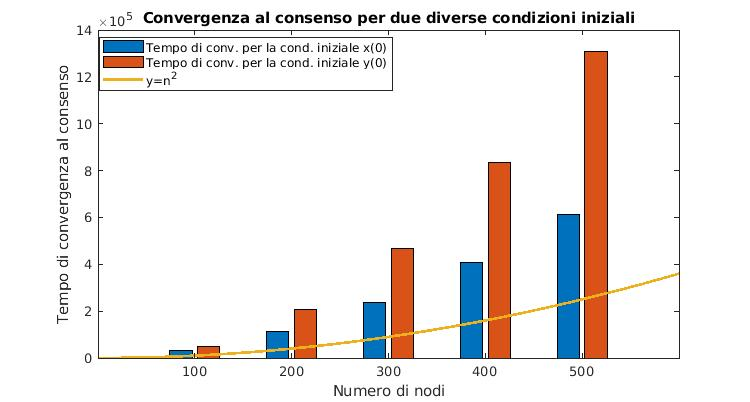
\includegraphics[scale=0.45]{figures/es1_plot.jpg}  
    \end{figure}

    Come si può notare la convergenza per la condizione \(y(0)\) scala molto più lentamente della condizione \(x(0)\) rispetto al numero di nodi. Entrambe sono tuttavia sopra il limite inferiore teorico calcolato al punto precedente. Questo fenomeno dipende dal fatto che nel caso di \(y(0)\) il consenso viene raggiunto utilizando come unico canale di comunicazione il singolo edge che collega i due cluster. Nel caso di \(x(0)\) questo non è necessario dal momento che le due opinioni sono distribuite uniformemente lungo tutto il grafo.

    \end{alphaparts}